\chapter{Sprites de Personajes} \label{Anexo:Personajes}
En este apéndice se presentan los \textit{sprites} creados durante la duración
del trabajo terminal.

%	====	Xolotl	====
\begin{figure}[H]
    \centering
    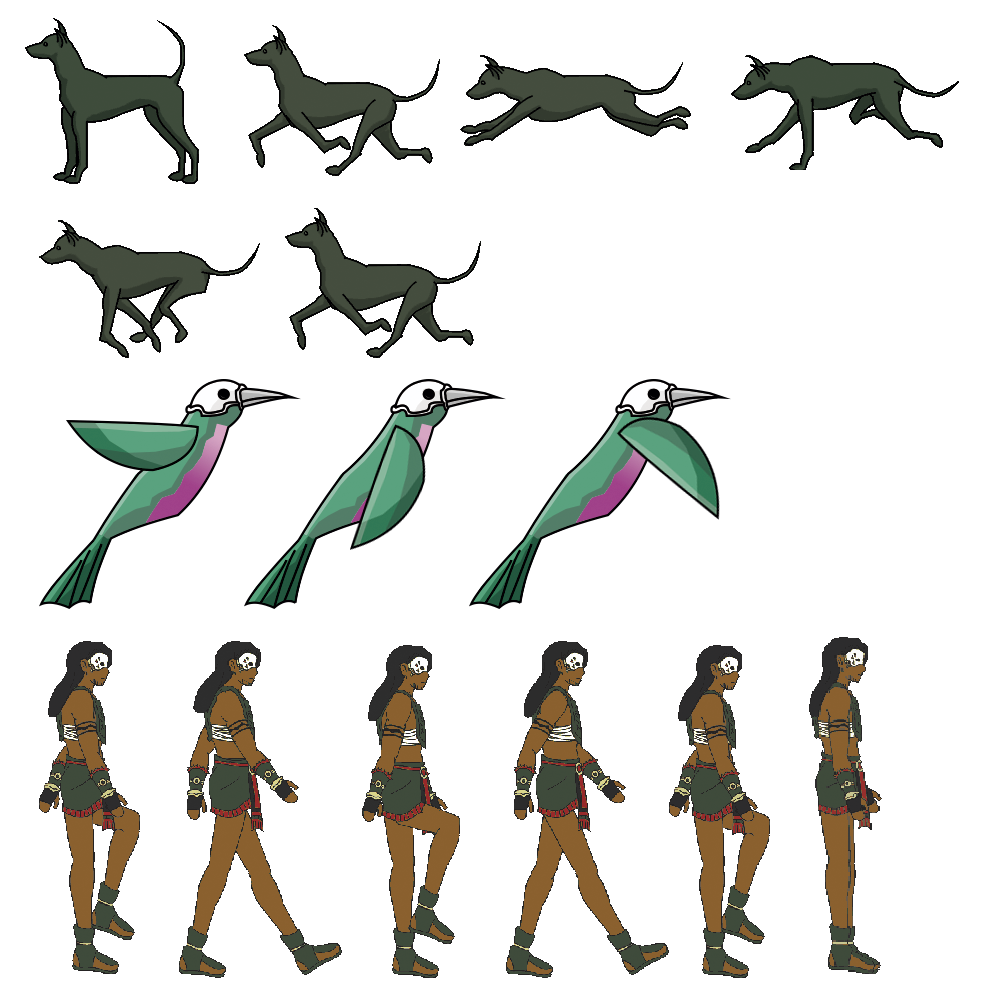
\includegraphics[width=0.40\textwidth]{Anexos/disenios/Xolotl.png}
    \caption{Sprites para las diferentes formas que toma Xólotl a lo largo del juego.}
    \label{fig:Xolotl}
\end{figure}

%	====	Enemigos normales	====
\begin{figure}[H]
    \centering
    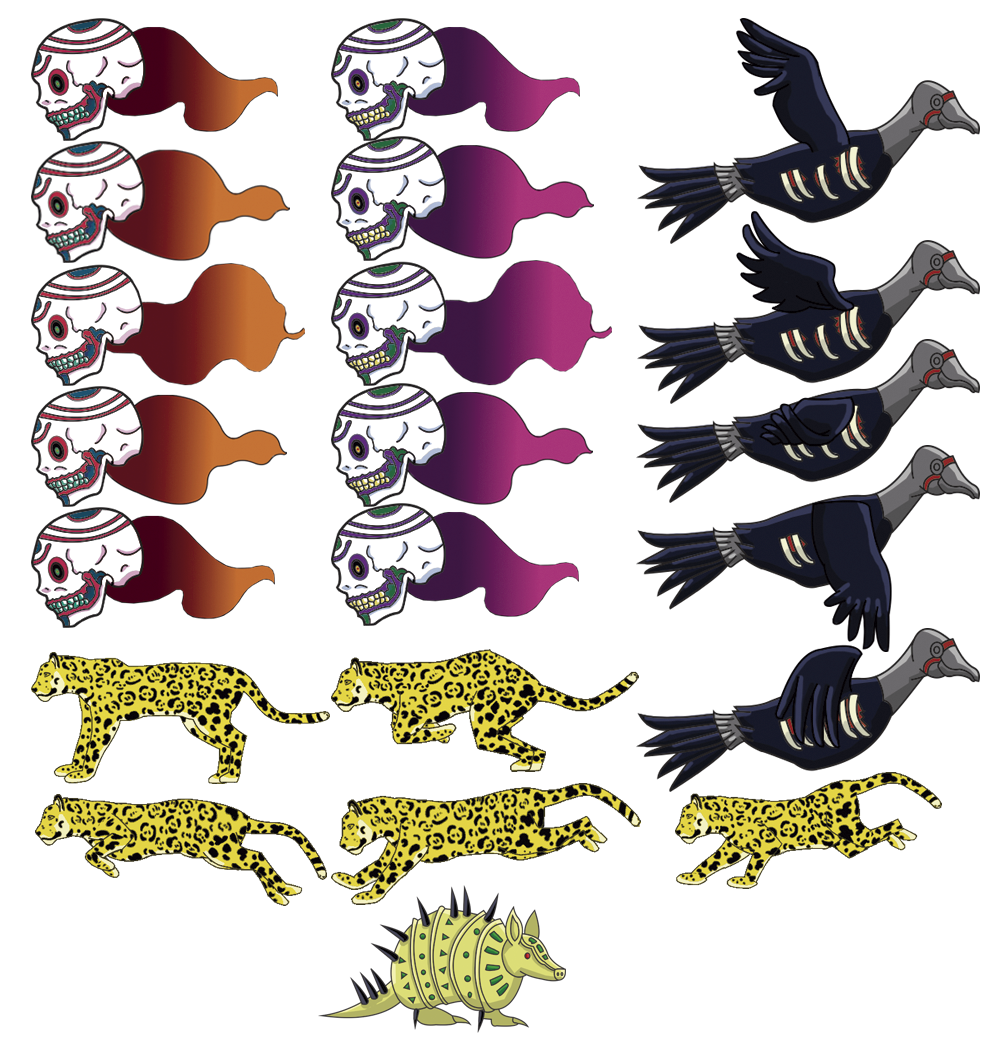
\includegraphics[width=0.40\textwidth]{Anexos/disenios/EnemigosNormales.png}
    \caption{Sprites para los enemigos normales del juego.}
    \label{fig:NorlmalEnemy}
\end{figure}

%	====	Jefes	====
\begin{figure}[H]
    \centering
    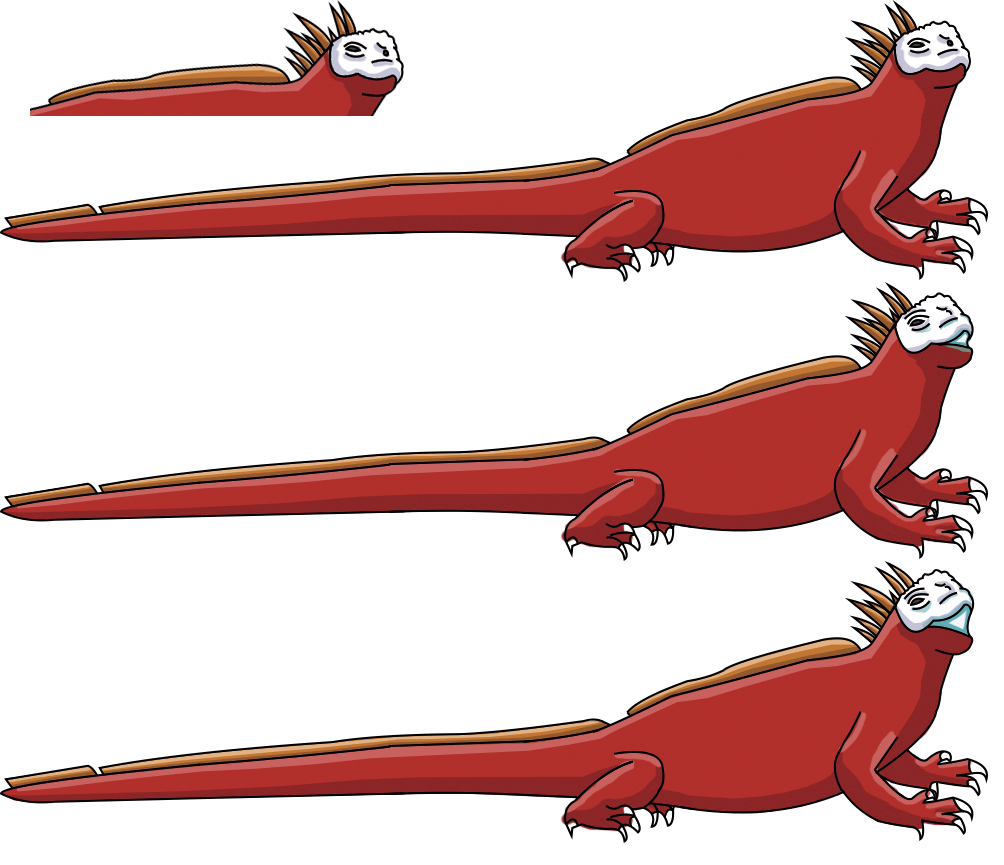
\includegraphics[width=0.40\textwidth]{Anexos/disenios/Xochitonal.png}
    \caption{Sprites de Xochitonal.}
    \label{fig:Xochitonal}
\end{figure}

\begin{figure}[H]
    \centering
    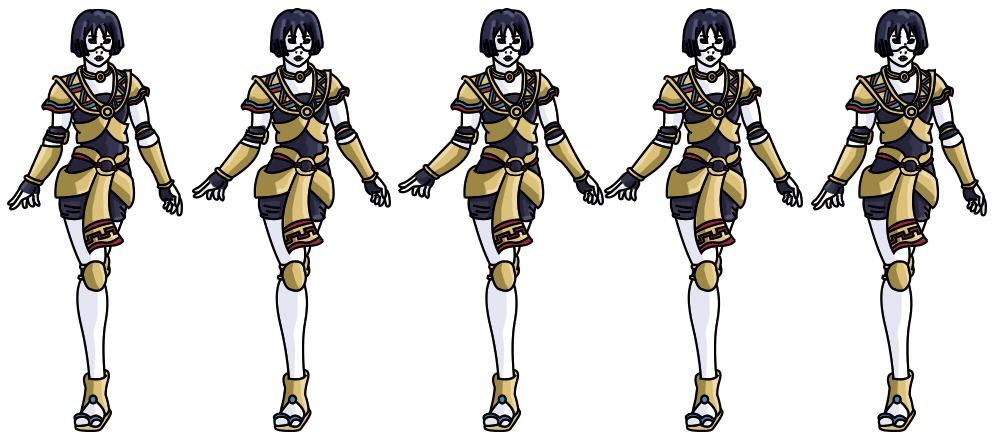
\includegraphics[width=0.40\textwidth]{Anexos/disenios/Itzpapalotl.png}
    \caption{Sprites de Itzpapálotl.}
    \label{fig:Itzpapalotl}
\end{figure}

\begin{figure}[H]
    \centering
    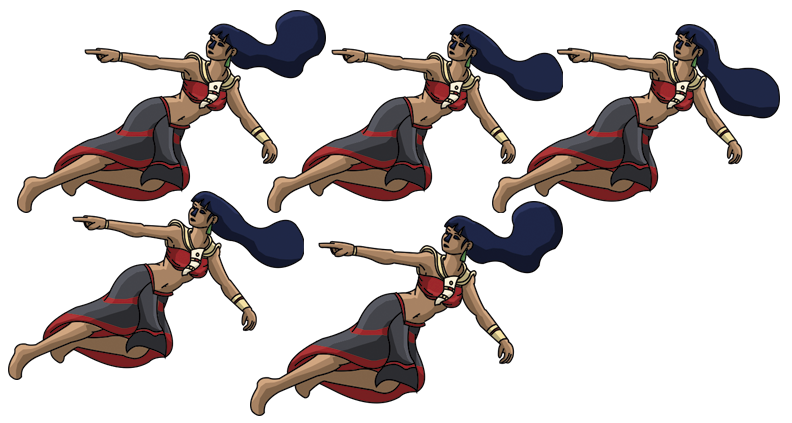
\includegraphics[width=0.40\textwidth]{Anexos/disenios/Tlazolteotl.png}
    \caption{Sprites de Tlazolteotl.}
    \label{fig:Tlazolteotl}
\end{figure}

\begin{figure}[H]
    \centering
    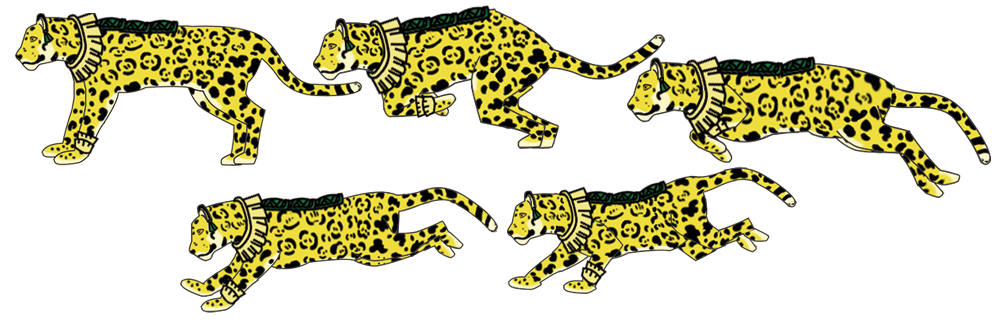
\includegraphics[width=0.50\textwidth]{Anexos/disenios/Tepeyollotl.png}
    \caption{Sprites de Tepeyollotl.}
    \label{fig:Tepeyollotl}
\end{figure}

\begin{figure}[H]
    \centering
    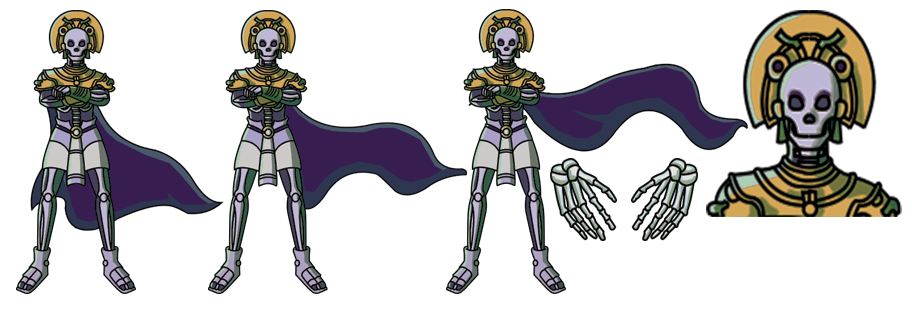
\includegraphics[width=0.50\textwidth]{Anexos/disenios/Mictlantecuhtli.png}
    \caption{Sprites de Mictlantecuhtli.}
    \label{fig:Mictlantecuhtli}
\end{figure}

%	====	Ataques Enemigos	====
\begin{figure}[H]
    \centering
    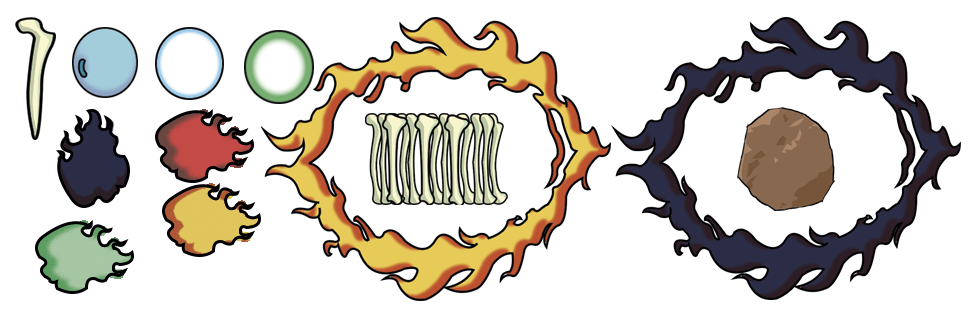
\includegraphics[width=0.50\textwidth]{Anexos/disenios/Ataques.png}
    \caption{Sprites de los ataques de los personajes.}
    \label{fig:Attack}
\end{figure}

%	====	Obstaculos	====
\begin{figure}[H]
    \centering
    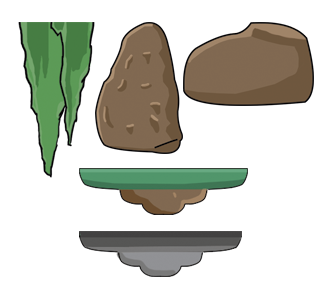
\includegraphics[width=0.3\textwidth]{Anexos/disenios/Obstaculos.png}
    \caption{Sprites de los obtáculos.}
    \label{fig:Obstacle}
\end{figure}

%	====	Objetos de fondo 	====
\begin{figure}[H]
    \centering
    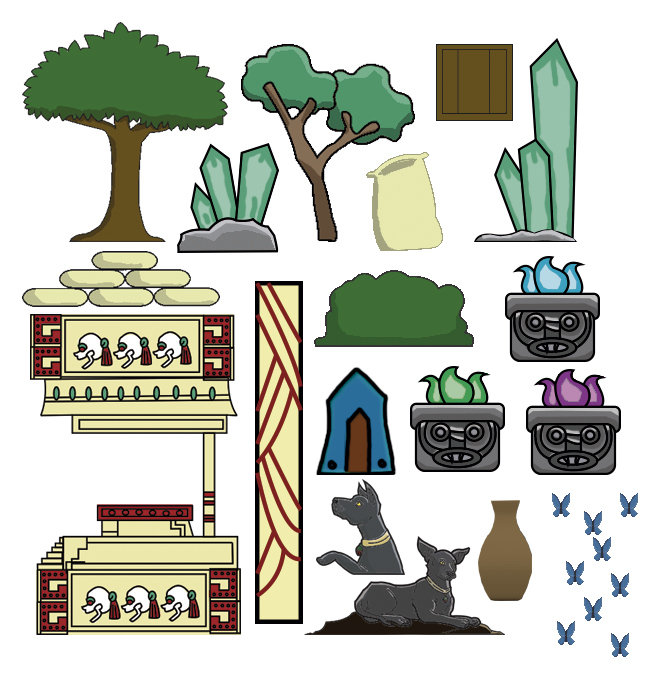
\includegraphics[width=0.50\textwidth]{Anexos/disenios/ObjetosFondo.png}
    \caption{Sprites de los objetos de fondo.}
    \label{fig:backObjects}
\end{figure}

%	====	check Point	====
\begin{figure}[H]
    \centering
    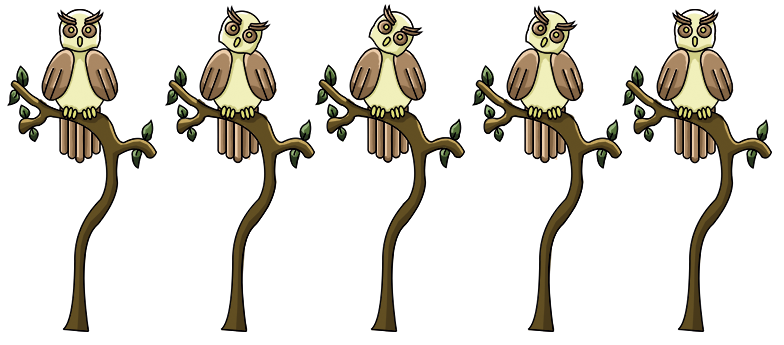
\includegraphics[width=0.50\textwidth]{Anexos/disenios/CheckPoint.png}
    \caption{Sprites de la animación del checkpoint.}
    \label{fig:backObjects}
\end{figure}

%	====	Ciudadanos	====
\begin{figure}[H]
    \centering
    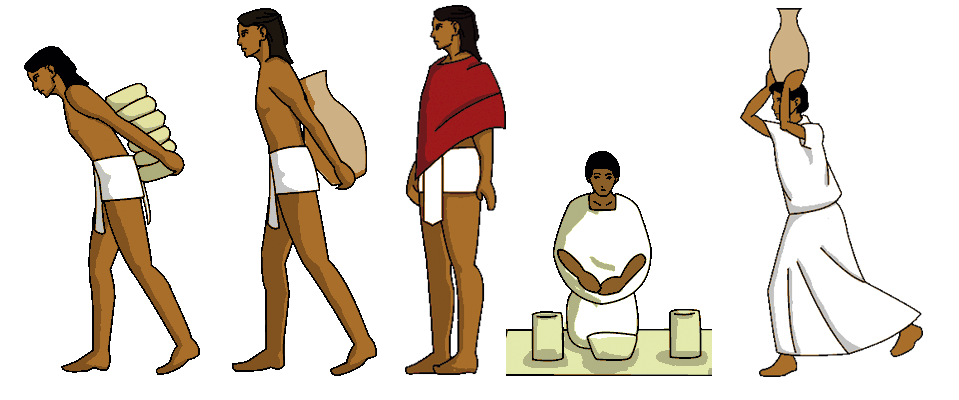
\includegraphics[width=0.50\textwidth]{Anexos/disenios/Ciudadanos.png}
    \caption{Sprites de los ciudadanos.}
    \label{fig:backObjects}
\end{figure}

%	====	iconos e ítems	====
\begin{figure}[H]
    \centering
    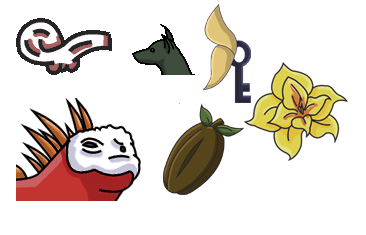
\includegraphics[width=0.30\textwidth]{Anexos/disenios/IconsItems.png}
    \caption{Sprites de los iconos e ítems.}
    \label{fig:backObjects}
\end{figure}

%	====	iconos e ítems	====
\begin{figure}[H]
    \centering
    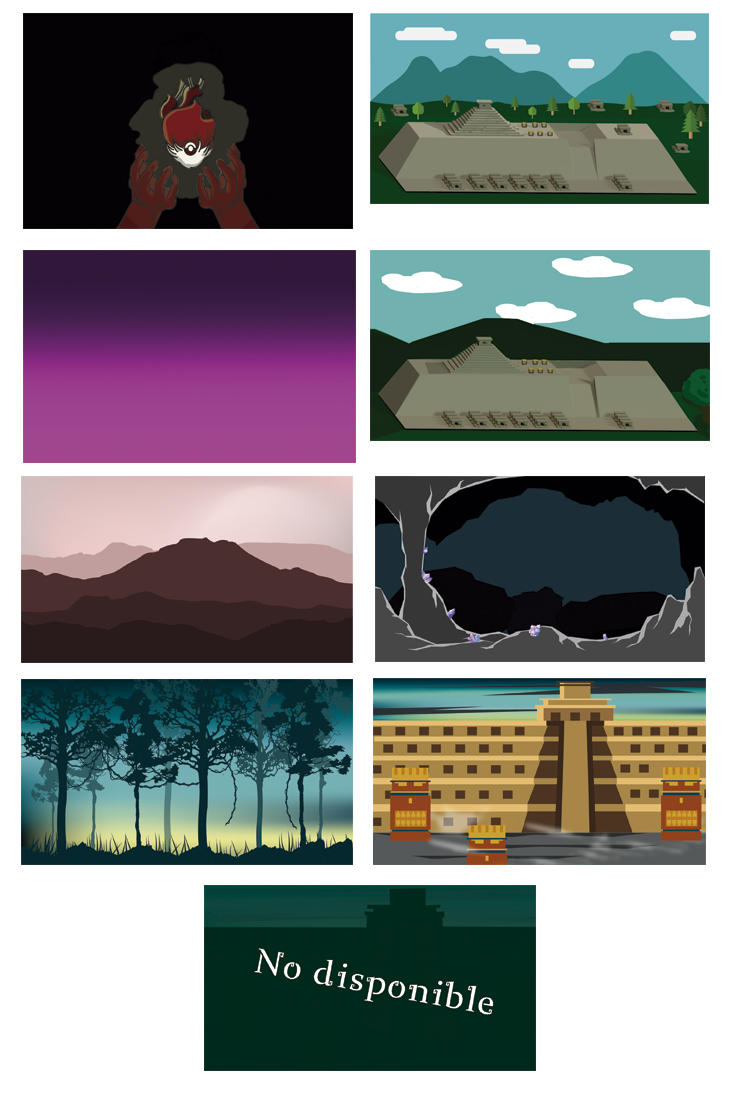
\includegraphics[width=0.50\textwidth]{Anexos/disenios/Fondos.png}
    \caption{Sprites de los findos de cada nivel.}
    \label{fig:BG}
\end{figure}

%	====	Mallinalli	====
\begin{figure}[H]
  		\centering
   		\subfigure[Sprites Malinalli para el primer nivel.] {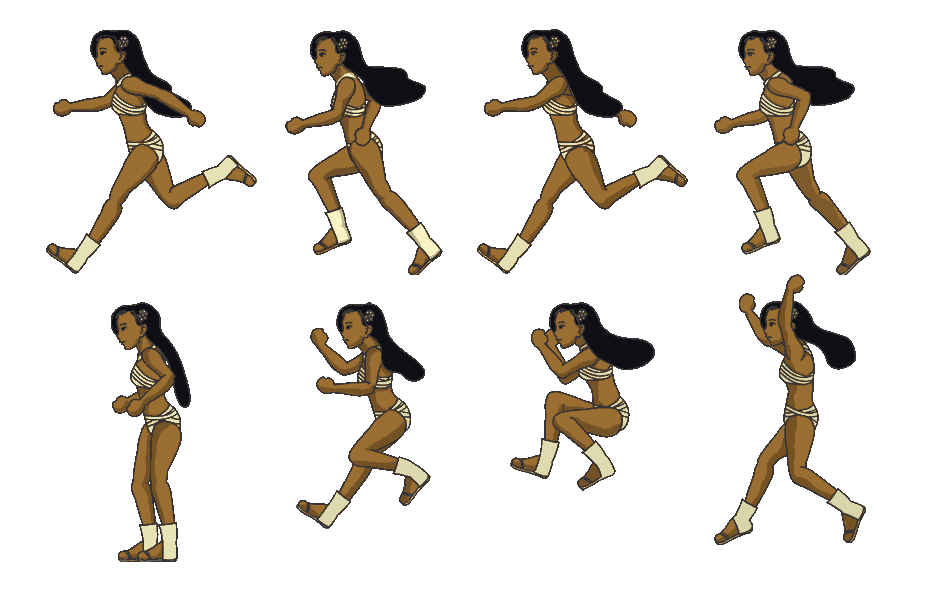
\includegraphics[width=0.3 \textwidth]{Anexos/disenios/MalinalliNormal.png}}
   
 		\subfigure[Sprites Malinalli de nado para el segundo nivel.]{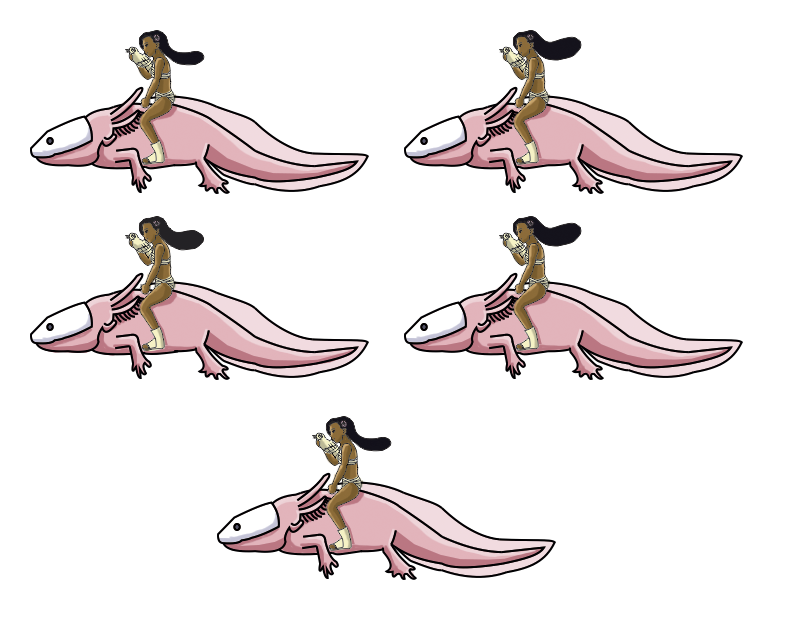
\includegraphics[width=0.3 \textwidth]{Anexos/disenios/MalinaliAjolote.png}}
 	
		\subfigure[Sprites Malinalli de salto para el segundo nivel.] {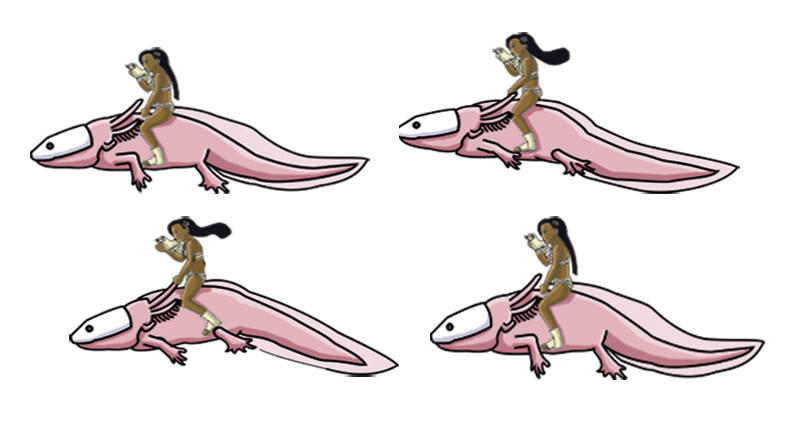
\includegraphics[width=0.3 \textwidth]{Anexos/disenios/MalinaliAjolotesalto.png}}
		
		\subfigure[Sprites Malinalli para los niveles posteriores al segundo nivel.] {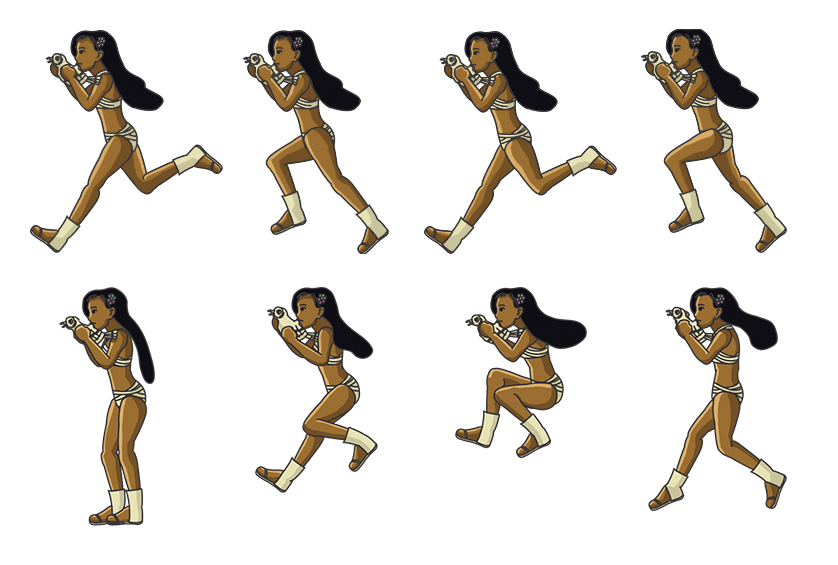
\includegraphics[width=0.3 \textwidth]{Anexos/disenios/MalinalliArma.png}}
		
  		\caption{Sprites del personaje jugable (Autoria propia)}
  		\label{fig:Malinalli}
\end{figure} 